Le \textit{back-office} d'une application web conçue pour gérer les données de la
recherche, à l'instar d'\aikon, est l'interface interne, non accessible
au public. Cette interface offre un espace de travail centralisé aux
chercheur.ses pour saisir, modifier, supprimer et organiser les données de
manière structurée. Elle assure également la gestion des utilisateur.rices et
des droits d'accès, garantissant ainsi la sécurité et la confidentialité
des informations.

L'enjeu majeur du \si \aikon est de structurer et d'uniformiser les
pratiques de recherche. Il entend se positionner comme outil efficace
pour la standardisation et l'optimisation des \textit{workflows}, offrant un
cadre méthodologique rigoureux. En regroupant l'ensemble des données de
recherche au sein d'une infrastructure commune, ce système rationalise
les opérations de gestion de données, réduit les risques de perte et facilite les recherches. Grâce à l'implémentation de
métadonnées descriptives, de formats de données standardisés et de
règles de validation, il assure la cohérence sémantique et structurelle
des données. Par ailleurs il facilite la collaboration, s'offrant comme
véritable ``laboratoire''. Enfin, en modélisant des protocoles d'analyse
des données, il contribue à la transparence de la recherche et la
reproductibilité des méthodes.

Ces buts peuvent être atteints en réfléchissant au design d'interface.

\hypertarget{avantages-des-interfaces-graphique-pour-la-recherche}{%
\subsection{Avantages des interfaces graphique pour la
recherche}\label{avantages-des-interfaces-graphique-pour-la-recherche}}

Une interface peut s'adapter à des utilisateur.rices aux profils variés.
Cela implique notamment de prendre en compte les questions de
multilinguisme (assurer \emph{a minima} le bilinguisme français et
anglais) et de littératie numérique. Comparée à des scripts
``artisanaux'', l'interface graphique présente l'avantage d'offrir une
abstraction des complexités techniques, permettant aux chercheur.ses de se
concentrer sur l'interprétation des résultats plutôt que sur la mise en
œuvre des algorithmes. De plus, elle assure une cohérence
méthodologique et facilite la collaboration en proposant un
environnement de travail unifié. Cette approche permet donc de gagner en
efficacité et en reproductibilité, tout en démocratisant l'utilisation
des outils de vision par ordinateur au sein de la communauté
scientifique.

Ainsi le \textit{back-office} doit se doter d'interfaces ergonomiques et faciles
à prendre en main. En effet, le public de chercheur.ses présente des profils
différents en terme de compétences numériques, c'est pourquoi il faut
veiller à l'intuitivité des
fonctionnalités.

\begin{kwote}
``Programmer ou savoir utiliser les logiciels~? Au cours d'une
expérience d'une base de données collaborative associée à un projet de
d'analyse d'images, les interfaces et la base de données ont été créées
par l'informaticien, avec les contraintes d'ergonomie et après conseil
des historien.nes. Cela a bien fonctionné. La conclusion à en tirer est que
les chercheur.ses doivent d'abord connaître les logiciels développés pour
eux, pas nécessairement savoir programmer. Des logiciels puissantes
existent, il n'est pas toujours nécessaire de réinventer la roue.
L'ignorance informatique des historien.nes doit être évitée, mais il est
nécessaire de disposer d'une bonne culture informatique, autorisant un
bon apprentissage des logiciels.''\footcite[p.35]{clavert_lhistorien_2012}
\end{kwote}

Une documentation a été rédigée pour aider les chercheur.ses à prendre la
plateforme en main~: elle est présentée en annexe \ref{doc_interfaces}.

\hypertarget{construction-logique-de-linterface-utilisateur.rice}{%
\subsection{Construction logique de l'interface
utilisateur.rice}\label{construction-logique-de-linterface-utilisateur.rice}}

La plateforme propose deux grands axes logiques de navigation,
correspondant à la gestion des documents d'un côté et à l'application
des traitements de vision artificielle de l'autre. Elle s'adapte alors
aux utilisateur.rices qui souhaitent utiliser l'\ia comme à ceux qui ont
essentiellement besoin d'un outil de gestion de données.

Cette séparation se reflète sur la page d'accueil présentant une
hiérarchie visuelle claire (deux blocs séparés 'Entités' et 'Mes Tâches').
Cette structure répétée dans la \textit{navbar} du \textit{header} présentant deux menus
déroulant distincts~: `Manage Documents' et `Computer Vision Tasks'.

\hypertarget{donner-acces-a-la-base-de-donnees-saisir-les-sources-et-les-consulter}{%
\subsubsection{Donner accès à la base de données~: saisir les sources et les
consulter}\label{donner-acces-a-la-base-de-donnees-saisir-les-sources-et-les-consulter}}

La plateforme \aikon est conçue pour agréger des données moissonnées à
partir de multiples \si. La structure de l'interface
d'administration, pensée pour accompagner le chercheur.se dans la
récupération des données et le peuplement de la base, est calquée sur le modèle
de données sous-jacent.

Le processus d'ajout de nouvelles entités (\wit, \ser, \wo) est
effectué via des formulaires conçus de manière à guider l'utilisateur.rice dans
la saisie des informations, permettant d'assurer la cohérence et la
qualité des métadonnées. Ces formulaires, directement liés à la
structure des tables de la base de données, proposent des champs
prédéfinis et des listes déroulantes ou de l'autocomplétion pour
normaliser les valeurs. Quand il rentre les métadonnées des entités
principales, le chercheur.se a accès à de nouveaux formulaires pour remplir
les tables de relation (lieux, langues, personnes, rôles\ldots),
constituant la liste des valeurs normalisées. Garantir la cohérence et
la qualité de la donnée implique tout de même de mettre en place des
règles de saisie strictes, éventuellement rassemblées dans une
documentation utilisateur.rice pour favoriser leur suivi et leur respect.

Le processus de saisie des métadonnées constitue en effet une étape
cruciale dans la construction et la valorisation d'une base de données
de recherche. Ces données descriptives, associées aux objets numériques
ou physiques, permettent d'en décrire précisément toutes les
caractéristiques (type, format, date de création, langue, auteurs, lieu,
institution de conservation, etc.)~; ce afin de faciliter ensuite la
trouvabilité. Des métadonnées riches et structurées permettent par la
suite de mettre en place des mécanismes de recherche plus performants
pour les chercheur.ses.

Les formulaires permettent aussi de décrire les liens entre les entités.
Le formulaire de saisie du \wit permet d'importer une ou plusieurs
\digits, et de renseigner un ou plusieurs \textit{Contents}. Le \textit{Content} est
associé à un \wo préalablement décrit et enregistré, et à un ou
plusieurs acteurs historiques. De cette manière, un \wo peut être relié
à plusieurs \wits et un \wit à plusieurs contenus donc
plusieurs \wos. L'entité \ser concerne plutôt le monde de l'imprimé,
elle est reliée à plusieurs \textit{Volume} d'une \textit{Édition} et le formulaire permet
d'importer une \digit par volume.

Chacune des entités principales dispose aussi d'une page qui liste
l'ensemble de ses enregistrements, permettant une circulation libre, sur
le mode de la découvrabilité. L'affichage de la liste des \wits,
\sers et \wos met en avant un ensemble de métadonnées liées à chaque
élément saisi. Cette organisation par entité permet de conserver la
cohérence avec la base de données relationnelle. Dans cette logique, les
pages de listes agrégeant les données conduisent aux notices
d'enregistrement unique, permettant de compléter ou modifier leurs
métadonnées.

Depuis ces interfaces, des fonctionnalités de recherche ont été mises en
place pour filtrer les résultats à l'aide de plusieurs critères. Les
formulaires de recherche amènent un autre mode de navigation, celui de
l'accès direct à la ressource.

\begin{figure}[H]
	\begin{center}
		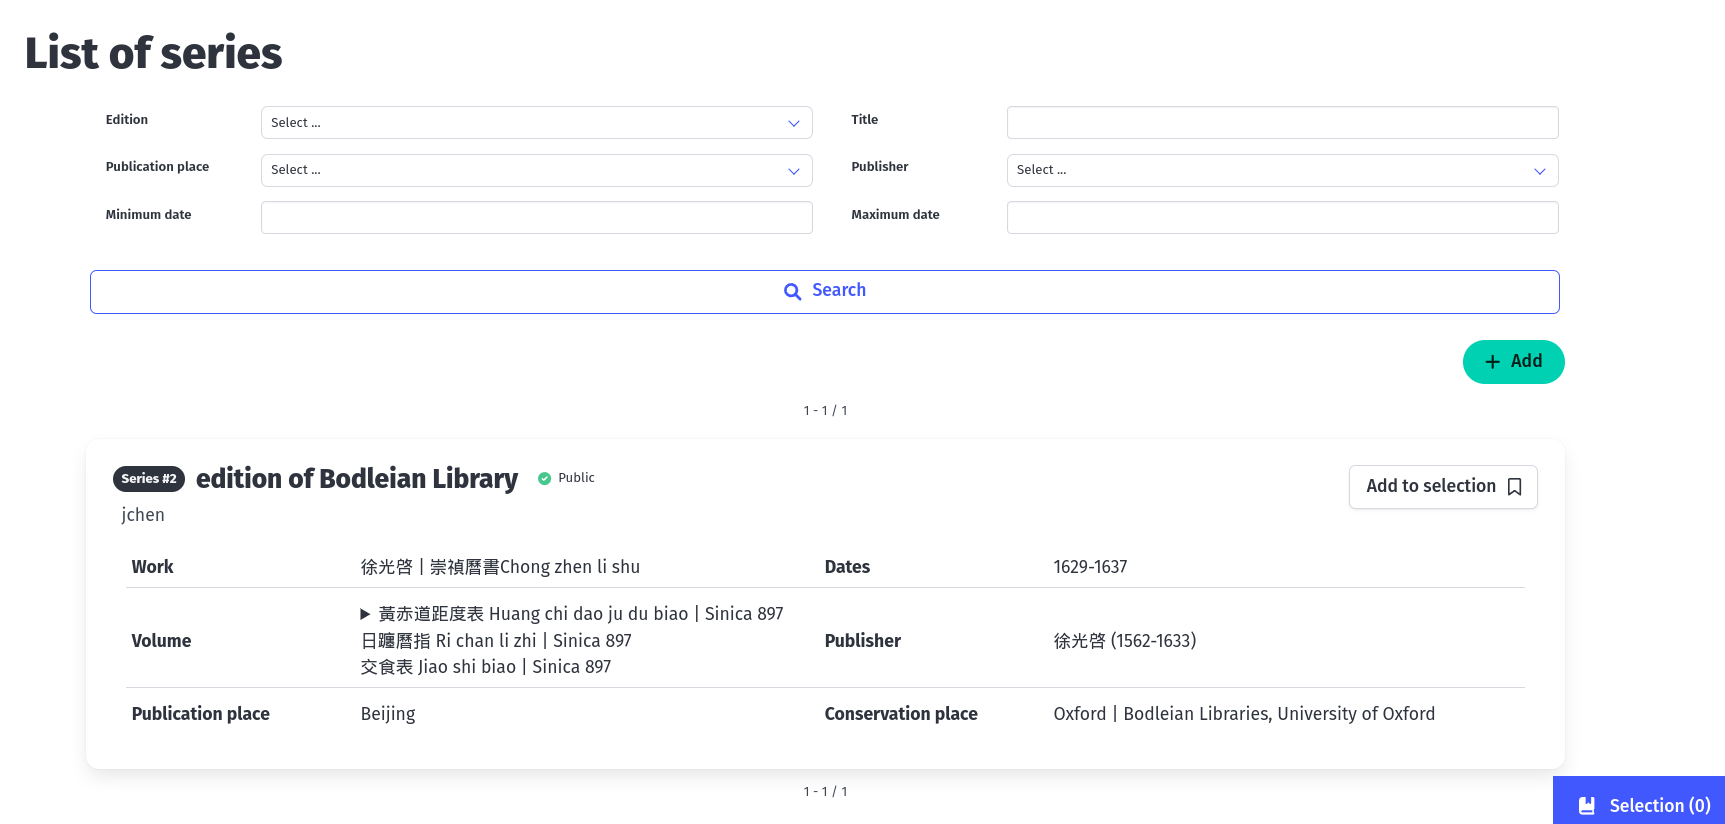
\includegraphics[height=7cm]{figues/serie_form_list.png}
	\end{center}
	\caption{Capture d'écran du formulaire de recherche des \sers.}
	\label{fig:form_recherche} \end{figure}

Le \textit{backend} administrateur constitue en ce sens une interface graphique
pour la base de données, les administrateurs pouvant rentrer les
données, accéder aux ressources qu'ils ont ajoutées, parcourir celles
ajoutées par d'autres, et ajuster les métadonnées.

\hypertarget{traitements-et-resultats}{%
\subsubsection{Traitements et Résultats}\label{traitements-et-resultats}}

La plateforme permet la sélection des entités dans les listes, et ainsi
la constitution de \dss dont le contenu est consultable et
modifiable dans une interface dédiée et accessible depuis la barre de
navigation. Ce sont sur ces ensembles de documents que peuvent être
appliqués des traitements de nature variée (export, recherche de
similarité, vectorisation etc.), déclenchés par l'utilisateur.rice. Le
formulaire de lancement est accessible directement sur l'interface de
consultation du \emph{set}, ainsi que via barre de navigation du header. Le
traitement d'un document unique passe aussi par la création d'un \ds.

Une fois un traitement effectué, l'utilisateur.rice reçoit un e-mail avec le
lien vers une page de résultats, encore en construction à l'été 2024.
Elle permettra de comparer les résultats d'un même traitement (par
exemple l'extraction) en fonction de différents paramètres (typiquement
en fonction de différents modèles).

Les résultats des traitements sont aussi accessibles à l'échelle d'un
\wit, via sa cartouche descriptive dans la page de liste. Un bouton
mène à une interface qui traite la donnée à un niveau de granularité
inférieur, le diagramme -- ou l'illustration découpée. L'utilisateur.rice
navigue entre l'affichage des régions extraites, des similarités et des
vectorisations dans différents onglets.

\begin{figure}[H]
          \begin{center}
          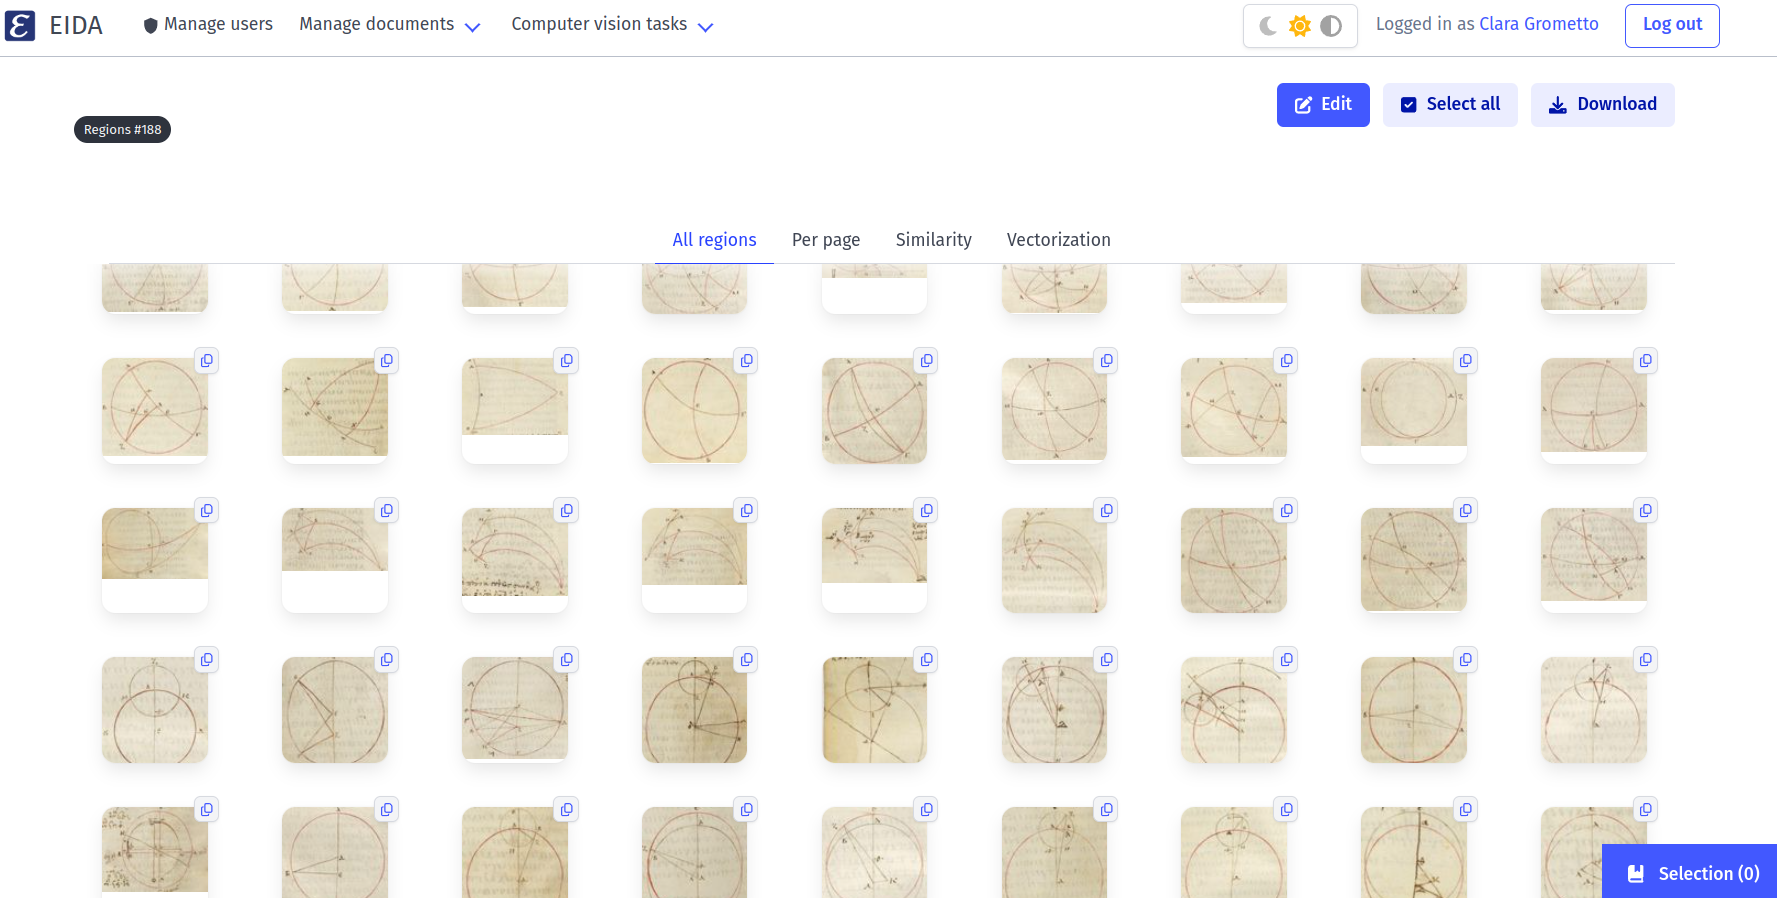
\includegraphics[height=7cm]{figues/dump_regions.png}
          \end{center}
          \caption{Capture d'écran de la visualisation des extractions type \textit{dump}, les onglets permettent de naviguer entre les interfaces de visualisation des résultats des traitements.}
          \label{fig:dump} \end{figure}

Pour l'extraction, deux visualisations sont proposées~: un affichage
synthétique de toutes les régions extraites (Fig. \ref{fig:dump}) et une représentation qui
les remet en contexte, présentant en regard la page de manuscrit
originale. C'est via ces visualisations que se fera la sélection des \rss (Fig. \ref{fig:selection}).

\begin{figure}[H]
	\begin{center}
		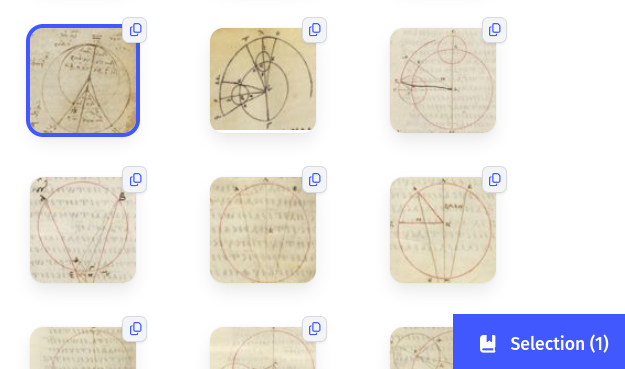
\includegraphics[height=5cm]{figues/selection.png}
	\end{center}
	\caption{Sélection des \rss.}
	\label{fig:selection} \end{figure}

Un onglet donne accès à une interface pour explorer les similarités
calculées par l'algorithme. Elle liste les témoins comparés. Sans
sélection, seules les zones extraites du témoin requête apparaissent.
L'utilisateur.rice peut afficher les similarités calculées pour un ou
plusieurs témoins, avec possibilité de filtrer selon les catégories
assignées par les chercheur.ses. Les 10 meilleurs scores, recalculés
dynamiquement, sont affichés par ordre décroissant.Un système de seuil
pour masquer les images avec un score bas, pourra également être
implémenté pour améliorer encore la lisibilité des résultats.
Actuellement, les similarités avec un score inférieur à 25 sont déjà
exclues pour réduire le temps de calcul. Le nombre de résultats affichés
pourrait aussi être ajusté. En résumé, cette interface est pensée pour
optimiser l'exploration et l'analyse des similarités détectés par le
modèle, grâce à des filtres superposables.

\begin{figure}[H]
          \begin{center}
          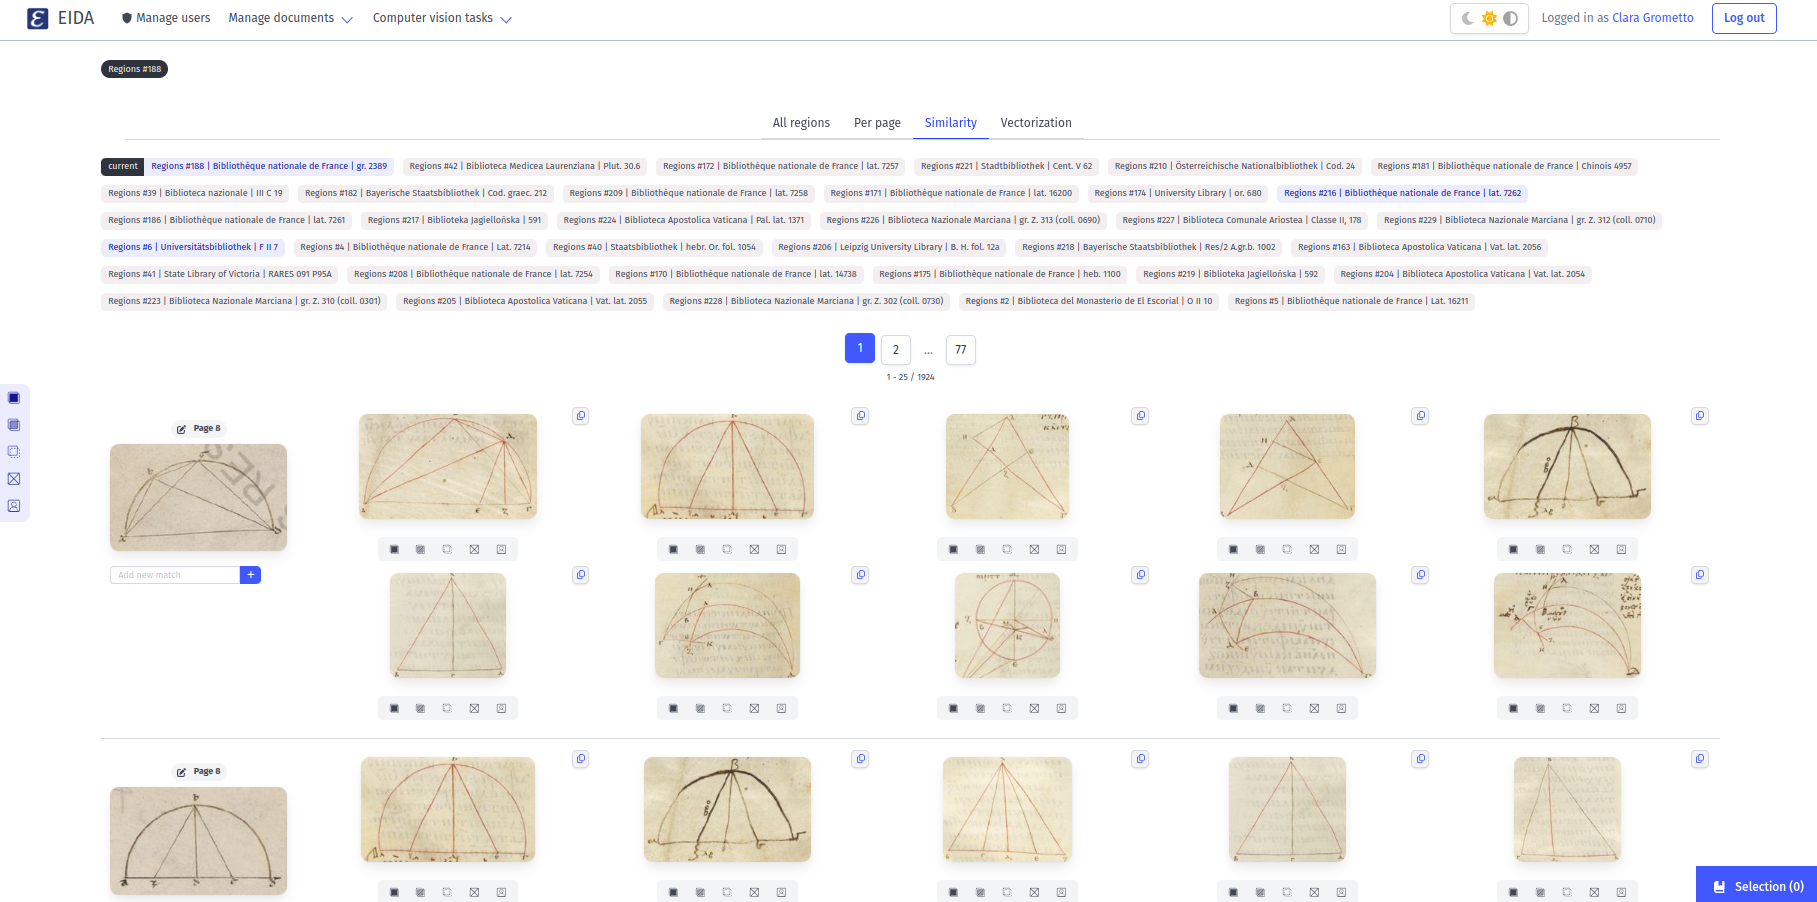
\includegraphics[height=8cm]{figues/sim.png}
          \end{center}
          \caption{Capture d'écran de l'interface de visualisation des similarités.}
          \label{fig:sim_interface} \end{figure}

La visualisation actuelle des vectorisations (Fig. \ref{fig:vecto_interface}) permet une exploration
préliminaire des données, mais reste sommaire (simple superposition du
\svg à l'image \jpeg). Des améliorations sont envisagées, notamment pour
implémenter l'export et la sélection en vue de l'établissement des
éditions.

\begin{figure}[H]
          \begin{center}
          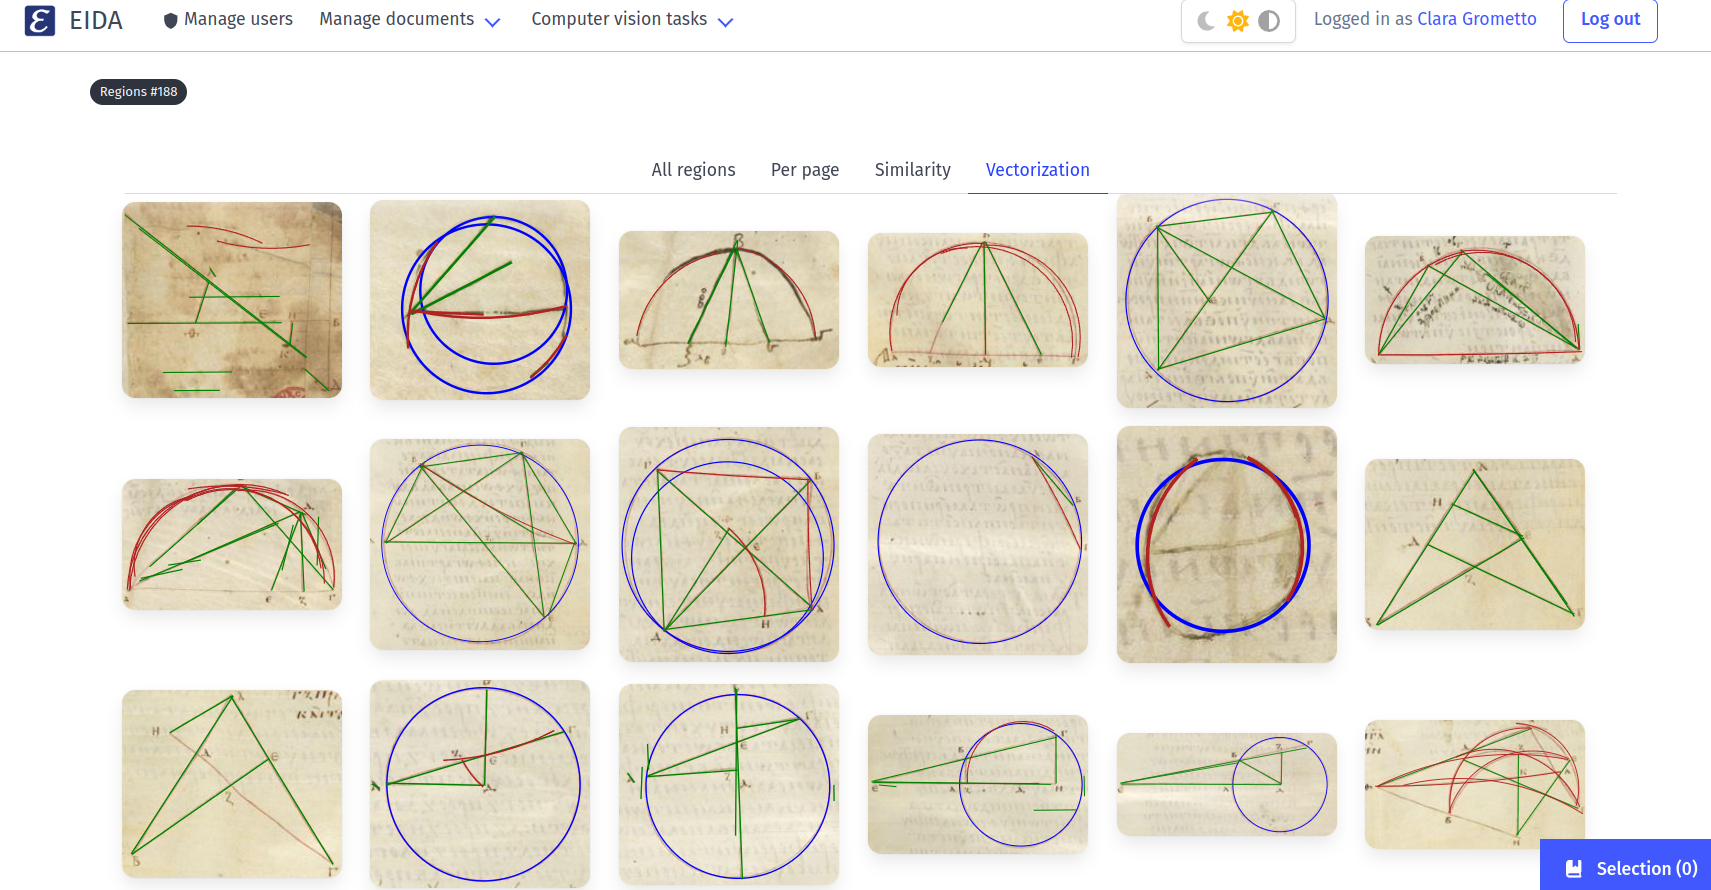
\includegraphics[height=6cm]{figues/vecto_interface.png}
          \end{center}
          \caption{Capture d'écran de l'interface d'affichage des vectorisations.}
          \label{fig:vecto_interface} \end{figure}

\hypertarget{annoter-et-exporter}{%
\subsubsection{Annoter et exporter}\label{annoter-et-exporter}}

S'inspirant des fonctionnalités proposées par la plateforme
e-scriptorium pour le texte, \aikon vise à offrir un environnement de
travail complet pour la sémantification et l'enrichissement des
documents numérisés présentant des éléments visuels. Grâce à la
plateforme, les utilisateur.rices peuvent donc non seulement effectuer des
traitements automatiques sur leurs données et les corriger, mais aussi
exporter les résultats dans différents formats interopérables, et donner
accès au \man \iiif annoté. Les premières données de prédiction
(\emph{silver data}), soumises à une validation humaine, viennent alors
enrichir des corpus d'entraînement (\emph{gold data}), permettant ainsi
d'affiner progressivement les modèles d'apprentissage profond et
d'améliorer la précision des résultats, alimentant une boucle de
rétroaction entre l'homme et la machine.

À ce titre, une attention particulière est portée à la vérification
manuelle des résultats. Sur l'interface de visualisation des similarités,
un champ est prévu pour ajouter manuellement celles qui auraient pu être
omises par les algorithmes. L'identifiant de l'extraction, copiable
depuis l'onglet de visualisation, est utilisé comme référence à verser
dans le champ de saisie.

L'évaluation du calcul de similarité entre images repose sur cinq
critères d'annotation prédéfinis (Fig. \ref{fig:cat}), permettant une qualification plus
précise du concept. Ces catégories, associés à chaque image similaire,
constituent des métadonnées importantes pour les chercheur.ses et servent
de filtre pour la visualisation des résultats. Mais surtout, l'ensemble
formé par les paires d'images annotées forme un corpus d'entraînement
pour améliorer les résultats du modèle.

\begin{figure}[H]
          \begin{center}
          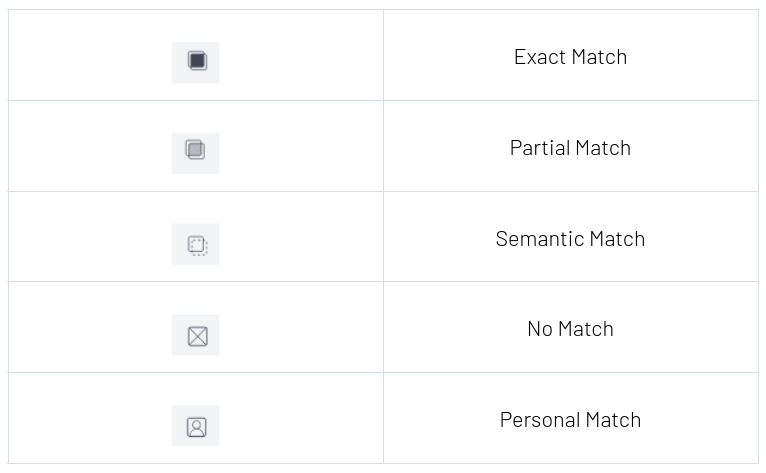
\includegraphics[height=6cm]{figues/recap_categories.png}
          \end{center}
          \caption{Récapitulatif des catégories de similarité et leurs icônes associées.}
          \label{fig:cat} \end{figure}

Il est par ailleurs possible de supprimer les extractions non
pertinentes depuis l'interface de visualisation de celles-ci (Fig. \ref{fig:correct}).
L'utilisateur.rice peut aussi accéder au visualiseur Mirador en cliquant sur
la page de manuscrit se trouvant en regard, afin d'y ajouter des annotations~:  diagrammes ou autre objet d'intérêt que l'algorithme aurait
manqué.

\begin{figure}[H]
          \begin{center}
          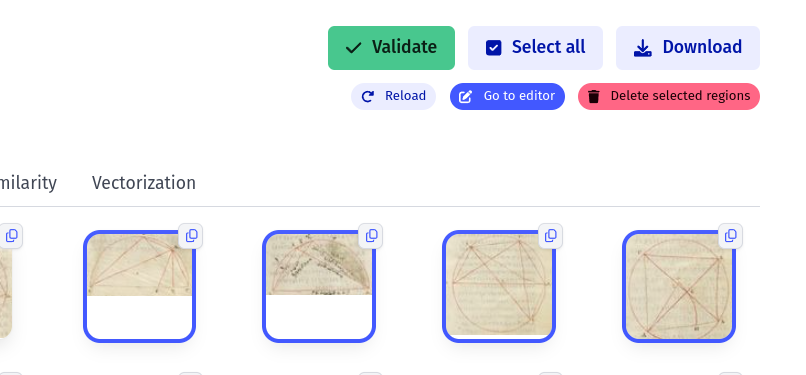
\includegraphics[height=6cm]{figues/annotation.png}
          \end{center}
          \caption{L'interface permet la validation des extractions.}
          \label{fig:correct} \end{figure}

La correction des prédictions s'inscrit donc dans un processus itératif
qui permet de construire des bases de données annotées et d'améliorer
les performance des modèles de classification, de détection, ou les calculs
de similarités. La prochaine étape consiste à implémenter un éditeur
\svg, intégrant des fonctionnalités de création et de modification de ce
format.

En conclusion, le \textit{back-office} d'une application web pour la gestion des
données est un outil qui peut améliorer l'efficacité, la qualité et la
transparence de la recherche. Il offre aux chercheur.ses un environnement
de travail collaboratif pour gérer les données et les intégrer dans une
chaîne de traitement basée sur des outils de vision par ordinateur. Le
parcours dans la plateforme est pensé pour guider les processus de
saisie et de traitement des données, et pour l'exploitation des
résultats.

La communauté scientifique accorde désormais une importance primordiale
à la visibilité et la réutilisabilité des bases de données\footcite{conference2023}, un enjeu majeur se situe donc dans l'ouverture et
l'accessibilité de celles-ci. La conception de l'interface utilisateur.rice
s'inscrit alors dans la perspective de son ouverture au public. Une
fois la base de données constituée et enrichie, elle a vocation à être
exposée. L'implémentation d'\apis assurera l'interopérabilité avec
d'autres plateformes et facilitera les échanges. En outre, la
perspective de l'exposition et la médiation des données impacte les
choix techniques concernant l'interface.